\subsubsection{Schaltungsaufbau} \label{subsubsec:schaltungsaufbau}
Ein EMI-Filter ist ein Netzwerk aus R, L, C Bauteilen und einem Transformator. 

Die Schaltung \ref{fig:orig_Schaltung} \nameref{fig:orig_Schaltung} zeigt den Filteraufbau, wie er der Aufgabenstellung zu entnehmen ist. Um das Gegentaktrauschen und das Gleichtaktrauschen bestimmen zu können, werden die beiden Schaltungsäquivalente gebildet. 
\begin{figure}[H]
	\centering
	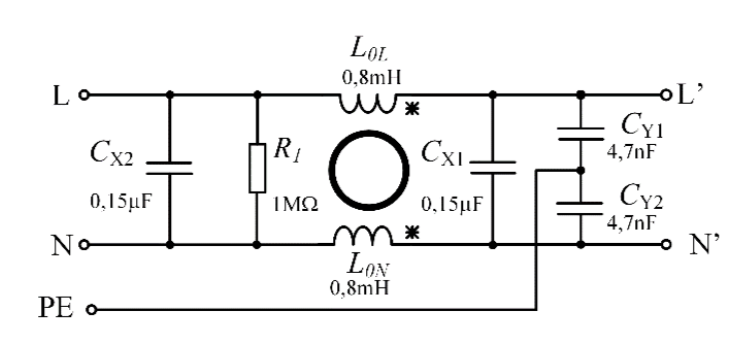
\includegraphics[width = 10cm]{orig_ElectricalCircuit.png}
	\caption{Original Schaltung \cite{aufgabenstellung}}
	\label{fig:orig_Schaltung}
\end{figure}


%TODO Die Schaltungsäquivalenzen müssen aufgeteilt werden und in die jeweiligen subsubsections gekippt werden
%TODO Reziprokzität einfügen
%TODO Allgemein EMI-Filter beschreiben
